\chapter{Analisis dan Perancangan}
\label{chap:Analisis dan Perancangan}

Pada bab ini, penulis akan menjelaskan apa saja yang dilakukan dalam pengembangan \textit{Agglomerative Hierarchical Clustering} untuk Spark. Pengembangan dilakukan untuk mencapai tujuan yaitu mendapatkan pola dari dataset yang diolah. Pola yang ingin didapatkan meliputi perhitungan rata-rata, nilai maksimum, nilai minimum dan nilai standar deviasi dari setiap attribut yang ada pada data. Selain itu, perlu didapatkan juga jumlah anggota pada setiap \textit{cluster} yang dihasilkan dari algoritma \textit{Agglomerative Hierarchical Clustering}.


\section{Analisis Perangkat Lunak}

Pada bagian ini akan dijelaskan analisis algoritma \textit{Agglomerative Hierarchical Clustering} pada MapReduce, kebutuhan perangkat lunak, dan masalah yang ingin diselesaikan. 

\subsection{Identifikasi Masalah}

Dalam bidang \textit{big data}, volume data yang sangat besar harus disimpan dalam tempat penyimpanan yang sangat besar. Volume data \textit{big data} dapat mencapai \textit{peta bytes}. Volume yang terlalu besar akan meningkatkan biaya dan menghabiskan tempat penyimpanan data. Volume data perlu direduksi agar menghemat tempat dan biaya.\\ 

Teknologi Hadoop MapReduce dan algoritma \textit{Agglomerative Hierarchical Clustering} dapat digabungkan sebagai solusi untuk mereduksi data. Algoritma \textit{Agglomerative} dapat mereduksi data dengan mengambil pola-pola dari \textit{clusters} yang dibentuk. Sistem terdistribusi Hadoop membantu dalam proses membagikan dan memecah tugas agar dapat dikerjakan secara parallel.  Dengan begitu, proses reduksi data dengan algoritma \textit{Agglomerative} akan lebih cepat. \\

Tetapi teknologi Hadoop masih terlalu lambat dalam mereduksi data. Hal ini disebabkan karena Hadoop banyak melakukan penulisan dan pembacaan kepada disk. Proses \textit{disk} I/O pada Hadoop sangat tinggi dan meyebabkan algoritma \textit{Agglomerative} berjalan sangat lambat pada Hadoop. Pada setiap tahap Hadoop akan menuliskan hasilnya kepada \textit{disk} dan akan dibaca kembali oleh tahap selanjutnya dari \textit{disk} seperti pada Gambar  ~\ref{fig:mapreducediagram}.\\

\begin{figure}[H]
    \centering  
    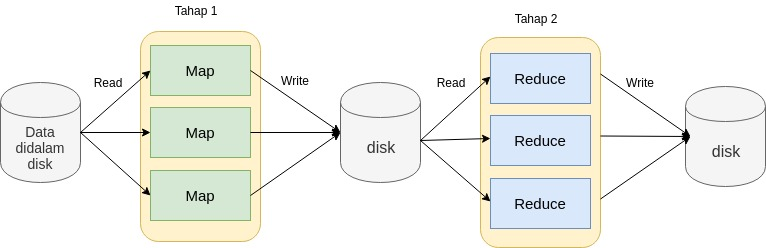
\includegraphics[scale=0.5]{mapreducediagram}  
    \caption[Gambar penulisan kepada disk di MapReduce]{Gambar penulisan kepada disk di MapReduce} 
    \label{fig:mapreducediagram} 
\end{figure}


Solusinya adalah menggabungkan teknologi terdistribusi lainnya dengan  algoritma \textit{Agglomerative} untuk mereduksi data. Spark, sistem terdistribusi yang menyimpan data pada memori dapat menggantikan Hadoop MapReduce. Kecepatan memori lebih cepat dibanding disk merupakan salah satu faktor mengapa Spark akan memproses data dengan kecepatan yang lebih tinggi.  Pembacaan han penulisan akan dilakukan kepada memori. Gambar ~\ref{fig:memorydiagram} adalah contoh ilustrasi tahap proses data di Spark. 
	
\begin{figure}[H]
    \centering  
    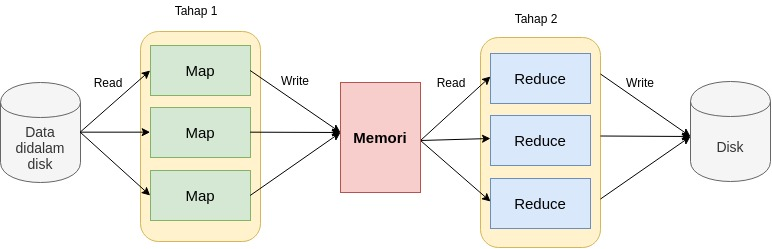
\includegraphics[scale=0.5]{memorydiagram}  
    \caption[Gambar penulisan kepada memori di Spark]{Gambar penulisan kepada memori di Spark} 
    \label{fig:memorydiagram} 
\end{figure}

\subsection{Kebutuhan Perangkat Lunak}

Dalam melakukan perancang perlu diketahui dulu kebutuhan perangkat lunak. Perangkat lunak yang dirancang harus dapat menghasilkan pola yang nantinya dapat dibandingkan dengan hasil pola dari perangkat lunak MapReduce. Pola yang dibutuhkan diantaranya:

\begin{enumerate}

\item Jumlah objek pada \textit{cluster}.

\item Nilai minimum setiap atribut pada \textit{cluster}.

\item Nilai maksimum setiap atribut pada \textit{cluster}.

\item Nilai rata-rata setiap atribut pada \textit{cluster}.

\item Nilai standar deviasi setiap atribut pada \textit{cluster}.
\end{enumerate}
 
\subsection{Analisis Agglomerative Hierarchical Clustering MapReduce}

\textit{Agglomerative Hierarchical Clustering} MapReduce dibagi menjadi dua bagian. Bagian pertama terkait tahap \textit{map} dan bagian kedua terkait tahap \textit{reduce}. Tahap \textit{map} akan dijelaskan dengan \textit{pseudocode} berikut ini \ref{alg:mapper}  

\begin{algorithm}[H]
	\DontPrintSemicolon\SetAlgoNoLine\LinesNumbered
	\SetKwInOut{Input}{Masukan}
	\SetKwInOut{Output}{Keluaran}
	\SetKwInOut{Desc}{Deskripsi}
	\Input{Data mentah (\textbf{TO)}); jumlah partisi (\textbf{n}) }
	\Output{\textit{key} = sebuah bilangan bulat $\epsilon$ \{1 ... $n$\}  \textit{value} = teks dari sekumpulan nilai atribut yang telah diproses sebelumnya}
	\Desc{memecah \textbf{TO} dengan memberi bilangan acak untuk setiap objek}
	\BlankLine
	\SetKwHangingKw{va}{\textbf{value} $\leftarrow$}
	\SetKwHangingKw{ke}{\textbf{key} $\leftarrow$}
	\SetKwHangingKw{hasil}{}
	\Begin{
		\va{membaca baris  dan memproses atributnya}
		\ke{sebuah bilangan acak $k$, dimana 1 $\leq$ $k$ $\leq$ $n$ }
		mengembalikan pasangan <\textit{key}, \textit{value}> sebagi hasil
	}
	
	
	\caption{Algoritma \textit{Mapper}}
	\label{alg:mapper}
\end{algorithm}


\section{Perancangan Perangkat Lunak}

Pada bagian ini, akan dijelaskan perancangan perangkat lunak.  Perancangan termasuk diagram \textit{use case}, skenario, diagram kelas, dan rancangan antarmuka. 

\subsection{Diagram Use Case dan Skenario}

Diagram \textit{use case} merupakan sebuah pemodelan untuk perilaku dari perangkat lunak yang akan dibuat. Diagram \textit{use case} digunakan untuk mengetahui fungsi apa saja yang ada dalam perangkat lunak. Fungsi-fungsi dari perangkat lunak akan dioperasikan oleh satu pengguna. Cara kerja dan perilaku dari perangkat lunak akan dijelaskan dalam bentuk diagram \textit{use case}. Diagram \textit{use case} dapat dilihat pada Gambar ~\ref{fig:usecase}.

\begin{figure}[H]
    \centering  
    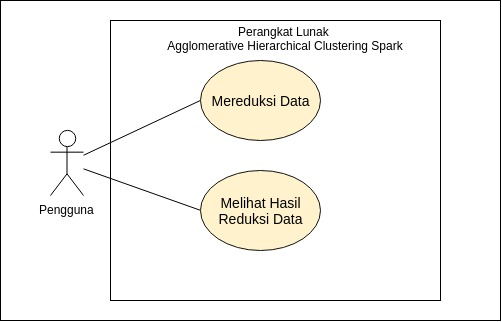
\includegraphics[scale=0.7]{usecase}  
    \caption[Gambar diagram \textit{use case} perangkat lunak \textit{Agglomerative Hierarchical Clustering}]{Gambar diagram \textit{use case} perangkat lunak \textit{Agglomerative Hierarchical Clustering}} 
    \label{fig:usecase} 
\end{figure}

Bedasarkan gambar diagram \textit{use case} diatas, berikut adalah skenario yang ada:

\begin{enumerate}

\item Nama \textit{use case}: Mereduksi data

\begin{itemize}
\item Aktor: Pengguna

\item Pre-kondisi: data yang akan diolah dimasukan kepada HDFS

\item Pra -kondisi: hasil reduksi disimpan pada HDFS

\item Deskripsi: Fitur untuk menjalankan program untuk mereduksi data

\item Langkah-langkah:

\begin{enumerate}

\item Pengguna mengisi JAR \textit{path}, \textit{input path}, dan \textit{output path}

\item Pengguna mengisi jumlah \textit{executor} dan besar \textit{executor memory}

\item Pengguna mengisi jumlah partisi, batas maksimum objek, tipe metode, dan \textit{cut-off distance} 

\item Pengguna menekan tombol \textit{submit}

\item Sitem melakukan pengolahan data dengan algoritma \textit{Agglomerative Hierarchical Clustering} pada \textit{cluster} Hadoop

\item Sistem membuka tab baru untuk melihat tahap dan progres program

\item Sistem menyimpan hasil reduksi pada HDFS
\end{enumerate}

\end{itemize}


\item Nama \textit{use case}: Melihat data

\begin{itemize}
\item Aktor: Pengguna

\item Pre-kondisi: data yang akan ditampilkan sudah disimpan pada HDFS

\item Pra -kondisi: menampilkan data yang ada pada HDFS

\item Deskripsi: fitur untuk melihat data hasil reduksi

\item Langkah-langkah:

\begin{enumerate}

\item Pengguna mengisi \textit{path} dimana data disimpan pada HDFS

\item Sistem menampilkan data-data pada direktori tersebut

\end{enumerate}

\end{itemize}

\end{enumerate}


\subsection{Diagram Kelas}

Pada bagian ini akan dijelaskan diagram kelas dari perangkat lunak. Diagram kelas dapat dilihat pada Gambar ~\ref{fig:classdiagram}.

\begin{figure}[H]
    \centering  
    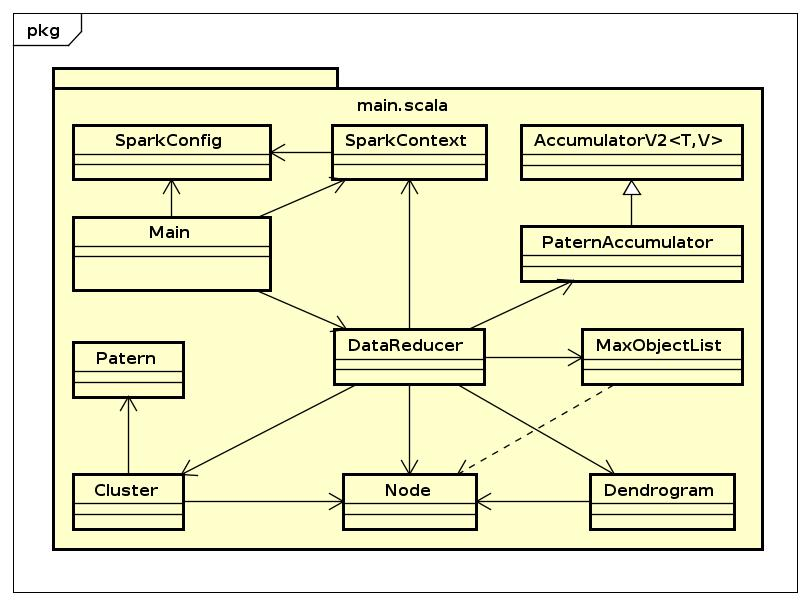
\includegraphics[scale=0.5]{classdiagram}  
    \caption[Gambar diagram kelas]{Gambar diagram kelas} 
    \label{fig:classdiagram} 
\end{figure}

Bedasarkan Gambar ~\ref{fig:classdiagram}, berikut ini adalah penjelasan kelas-kelas yang digunakan:

\begin{itemize}

\item \textbf{Main, Spark Config, dan Spark Context}\\

\begin{figure}[H]
    \centering  
    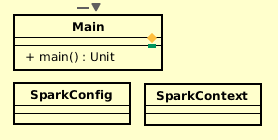
\includegraphics[scale=0.75]{maindiagram}  
    \caption[Gambar kelas Main, SparkConfig, SparkContext]{Gambar kelas Main, SparkConfig, SparkContext} 
    \label{fig:maindiagram} 
\end{figure}

Berikut adalah penjelasan dari ketiga kelas pada Gambar ~\ref{fig:maindiagram}:

\begin{itemize}

\item Main: kelas Main memiliki \textit{method main}  yang merupakan titik masuk dari program. \textit{Method} ini merupakan \textit{method} pertama yang akan dieksekusi ketika program dijalankan.

\item SparkConfig: kelas SparkConfig digunakan untuk mengatur konfigurasi untuk Spark. Pengaturan nama aplikasi, jumlah \textit{core}, besar \textit{memory}, dan lainya dapat diatur pada kelas ini.

\item SparkContext: kelas ini merupakan titik masuk untuk layanan-layan dari Apache Spark.\\

\end{itemize}


\item \textbf{DataReducer}\\

\begin{figure}[H]
    \centering  
    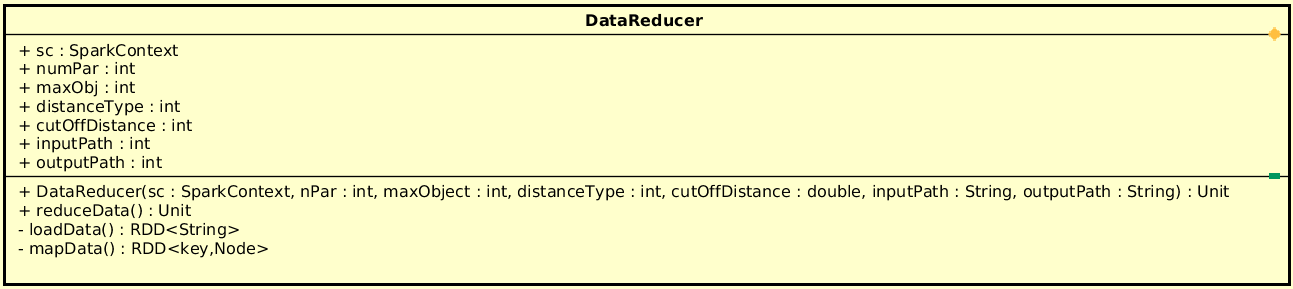
\includegraphics[scale=0.5]{datareducer}  
    \caption[Gambar kelas DataReducer]{Gambar kelas DataReducer} 
    \label{fig:datareducer} 
\end{figure}

Kelas DataReducer dirancang untuk memproses data. Proses reduksi secara parallel dilakukan pada kelas ini. Proses pemuatan dan penyimpanan data dilakukan pada kelas ini. Bedasarkan Gambar ~\ref{fig:datareducer}, berikut adalah penjelasan dari \textit{methods} pada kelas DataReducer:

\begin{enumerate}

\item loadData: \textit{method} untuk memuat data bedasarkan \textit{intput path} yang diberikan.

\item mapData: \textit{method} untuk memisahkan atribut dan membungkus attribut dalam objek Node agar lebih mudah diproses. \textit{Method} ini akan mengembalikan RDD bertipe Node.  

\item  reduceData: \textit{method} dimana proses reduksi data secara parallel terjadi. Data akan dipecah menjadi beberapa partisi pada method ini. Partisi ini akan diproses secara parallel. Method ini juga bertangung jawab untuk meyimpan pola hasil reduksi kepada HDFS.\\

\end{enumerate}


\item \textbf{Dendrogram}\\

\begin{figure}[H]
    \centering  
    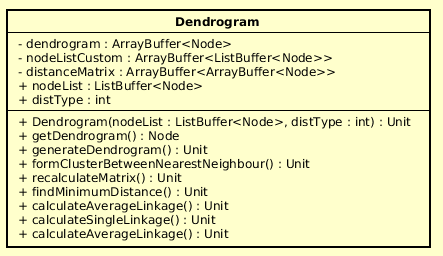
\includegraphics[scale=0.6]{dendrogramdiagram}  
    \caption[Gambar kelas Dendrogram]{Gambar kelas Dendrogram} 
    \label{fig:dendrogramdiagram} 
\end{figure}

Kelas Dendrogram dirancang untuk memproses data dan membangun dendrogram sesuai algoritma \textit{Agglomerative Hierarchical Clustering}. Bedasarkan Gambar ~\ref{fig:dendrogramdiagram}, berikut adalah penjelasan \textit{methods} pada kelas Dendrogram:

\begin{enumerate}
\item getDendrogram: \textit{method} ini mengembalikan dendrogram.

\item generateDendrogram: \textit{Method} untuk membangun dendrogram bedasarkan algoritma \textit{Agglomerative Hierarchical Clustering}. 

\item formClusterBetweenNearestNeighbour: method untuk menggabungkan \textit{cluster} terdekat.

\item recalculateMatrix: \textit{method} untuk menghitung ulang matriks jarak.

\item findMinimumDistance: \textit{method} untuk mencari jarak minimum antara dua \textit{cluster}.

\item calculateCentroidLinkage: method untuk mencari jarak antara centorid dua cluster.

\item calculateSingleLinkage: method untuk mencari jarak minimum antara dua cluster.

\item calculateCompleteLinkage: method untuk mencari jarak maksimum antara dua cluster.

\item calculateDistance: method untuk mencari jarak antara dua buah Node bedasarkan atributnya.\\
 
\end{enumerate}


\item \textbf{Cluster}\\

\begin{figure}[H]
    \centering  
    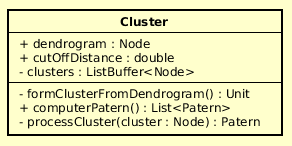
\includegraphics[scale=0.6]{clusterdiagram}  
    \caption[Gambar kelas Cluster]{Gambar kelas Cluster} 
    \label{fig:clusterdiagram} 
\end{figure}

Kelas Cluster dirancang untuk mengolah mengolah\textit{cluster} untuk menghasilkan pola dengan memotong \textit{cluster}. Bedasarkan Gambar ~\ref{fig:clusterdiagram}, berikut adalah penjelasan \textit{methods} pada kelas Cluster:

\begin{enumerate}

\item formClusterFromDendrogram: method ini bertugas untuk memotong \textit{dendrogram} menjadi beberapa \textit{cluster}.

\item computePatern: method untuk mengolah potongan-potongan \textit{cluster} menjadi pola dengan memanggil \textit{method} processCluster.

\item processCluster: method untuk memproses \textit{cluster} dan membuat pola bedasarkan atribut-atribut pada \textit{cluster}.\\
 
\end{enumerate}


\item \textbf{MaxObjectList}\\

\begin{figure}[H]
    \centering  
    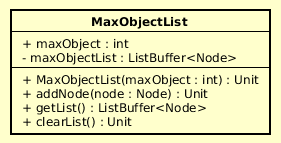
\includegraphics[scale=0.6]{maxobjlistdiagram}  
    \caption[Gambar kelas MaxObjectList]{Gambar kelas MaxObjectList} 
    \label{fig:maxobjlistdiagram} 
\end{figure}

Kelas MaxObjectList dirancang untuk membatasi jumlah objek yang akan diolah pada kelas Dendrogram. Bedasarkan Gambar ~\ref{fig:clusterdiagram}, berikut adalah penjelasan \textit{methods} pada kelas MaxObjectList:

\begin{enumerate}

\item addNode: method untuk menambahkan Node pada pada \textit{list}

\item getList: method ini mengembalikan \textit{list} berisi objek Node.

\item clearList: method untuk mengosongkan \textit{list}.\\
\end{enumerate}

\item \textbf{Patern}\\

\begin{figure}[H]
    \centering  
    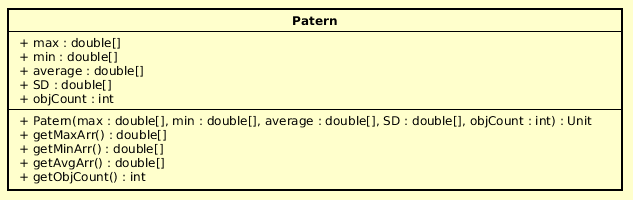
\includegraphics[scale=0.6]{paterndiagram}  
    \caption[Gambar kelas Patern]{Gambar kelas Patern} 
    \label{fig:paterndiagram} 
\end{figure}

Kelas Patern dirancang untuk merepresentasikan pola pada \textit{cluster}. Bedasarkan Gambar ~\ref{fig:clusterdiagram}, berikut adalah penjelasan \textit{methods} pada kelas MaxObjectList:

\begin{enumerate}

\item getMaxArr: \textit{method} ini mengembalikan \textit{array} berisi nilai maksimum dari setiap atribut.

\item getMinArr: \textit{method} ini mengembalikan \textit{array} berisi nilai minimum dari setiap atribut.

\item getAvgArr: \textit{method} ini mengembalikan \textit{array} berisi nilai rata-rata dari setiap atribut.

\item getSDArr: \textit{method} ini mengembalikan \textit{array} berisi nilai standar deviasi dari setiap atribut.

\item getObjCount: \textit{method} ini mengembalikan jumlah objek.\\
 
\end{enumerate}



\item \textbf{PaternAccumulator dan AccumulatorV2}\\

\begin{figure}[H]
    \centering  
    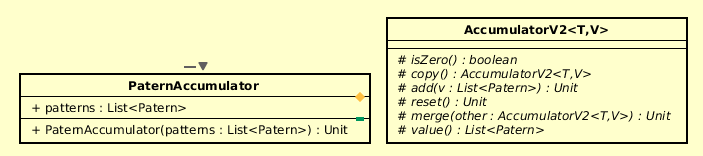
\includegraphics[scale=0.6]{paternaccumulatordiagram}  
    \caption[Gambar kelas PaternAccumulator dan AccumulatorV2]{Gambar kelas PaternAccumulator dan AccumulatorV2} 
    \label{fig:paternaccumulatordiagram} 
\end{figure}

Kelas PaternAccumulator dirancang untuk mengumpulkan pola-pola hasil reduksi. Kelas ini merupakan anak dari kelas abstrak \textit{AccumulatorV2} yang setiap \textit{method} harus di-\textit{override} pada kelas anaknya.  Bedasarkan Gambar ~\ref{fig:paternaccumulatordiagram}, berikut adalah penjelasan \textit{methods} pada kelas PaternAccumulator:

\begin{enumerate}

\item isZero: \textit{method} untuk mengetahui apakah list \textit{masih} kosong atau tidak.

\item copy: \textit{method} untuk menduplikat objek PaternAccumulator.

\item add: \textit{method} untuk menambahkan \textit{list} berisi pola-pola.

\item merge: \textit{method} untuk menggabungkan dua objek PaternAcumulator menjadi satu.\\

\end{enumerate}


\item \textbf{Node}\\

\begin{figure}[H]
    \centering  
    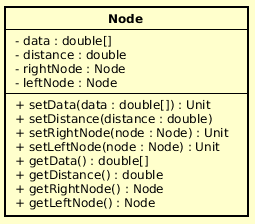
\includegraphics[scale=0.6]{nodediagram}  
    \caption[Gambar kelas Node]{Gambar kelas Node} 
    \label{fig:nodediagram} 
\end{figure}

Kelas Node digunakan untuk membentuk pohon yang merepresentasikan \textit{dendrogram}. Selain itu kelas ini digunakan untuk merepresentasikan anggota pada \textit{cluster}.  Bedasarkan Gambar ~\ref{fig:nodediagram}, berikut adalah penjelasan \textit{methods} pada kelas Node:

\begin{enumerate}

\item setData: \textit{method} untuk memasukan nilai-nilai atribut.

\item setDistance: \textit{method} untuk megubah nilai jarak.

\item setRightNode: \textit{method} untuk menambahkan anak kanan Node.

\item setLeftNode: \textit{method} untuk menambahkan anak kiri Node.

\item getData: \textit{method} ini mengembalikan nilai-nilai atribut.

\item getDistance: \textit{method} ini mengembalikan jarak.

\item getRightNode: \textit{method} ini mengebalikan anak belah kanan dari Node.

\item getLeftNode: \textit{method} ini mengebalikan anak belah kiri dari Node.

\end{enumerate}



\end{itemize}




\subsection{Rancangan Antarmuka}